\documentclass{article}
\usepackage[]{float,latexsym,times}
\usepackage{amsfonts,amstext,amsmath,amssymb,amsthm}
\usepackage{mathrsfs}
\usepackage{bbm}
\usepackage{mathtools} % for dcases
\usepackage{paralist}  % for inparaenum
\usepackage{blkarray}  % for block matrices
\usepackage{pgf,tikz}

\usepackage[margin=0.8in]{geometry}
\usepackage{hyperref}

\newcommand{\ignore}[1]{}

% Math notation
\newcommand{\set}[1]{\left\{#1\right\}}
\newcommand{\bigset}[1]{\big\{#1\big\}}
\newcommand{\Bigset}[1]{\Big\{#1\Big\}}
\newcommand{\slfrac}[2]{\left. #1 \middle/ #2 \right.}
\newcommand{\ceil}[1]{\left\lceil #1 \right\rceil}
\newcommand{\floor}[1]{\left\lfloor #1 \right\rfloor}

% Probability notation
\renewcommand{\mspace}[1]{\mathscr{#1}}
\newcommand{\algebra}[1]{\mathscr{#1}}
\newcommand{\prob}[1]{\mathbf{#1}}
\newcommand{\cond}[2]{\left. {#1} \, \middle | \, {#2} \right.}
\newcommand{\ci}{\perp\!\!\!\perp}             % Conditional independence.
%\renewcommand{\Pr}{\operatorname{\mathbf{P}}}  % probability measure
\DeclareMathOperator{\EV}{\mathbf{E}}          % expected value
\DeclareMathOperator{\Var}{\mathbf{Var}}       % variance
\DeclareMathOperator{\Cov}{\mathbf{Cov}}       % covariance

% Probability distributions
\newcommand{\Binomial}{\mathrm{Bin}}

% Well-known sets
\newcommand{\tinyinfty}{\infty} % or {\scriptscriptstyle \infty}
\newcommand{\tinyzero}{0} % or {\scriptscriptstyle 0}
\newcommand{\One}{\mathchoice{\rm 1\mskip-4.2mu l}{\rm 1\mskip-4.2mu l}{\rm 1\mskip-4.6mu l}{\rm 1\mskip-5.2mu l}}
\newcommand{\Naturals}{\mathbb{N}}
\newcommand{\Reals}{\mathbb{R}}

% Styles
\renewcommand{\le}{\leqslant}
\renewcommand{\leq}{\leqslant}
\renewcommand{\ge}{\geqslant}
\renewcommand{\geq}{\geqslant}
\newcommand{\overwr}{\leftarrow}

% Short-hand notation
\newcommand{\cA}{\mathcal{A}}
\newcommand{\cG}{\mathcal{G}}
\newcommand{\cH}{\mathcal{H}}
\newcommand{\cI}{\mathcal{I}}
\newcommand{\cJ}{\mathcal{J}}

% Document-specific

% Spaces of:
\newcommand{\Sutype}{\mathcal{U}} % Unit types
\newcommand{\Sctype}{\mathcal{C}} % Camp types
\newcommand{\Sgtype}{\mathcal{G}} % Unit groups
\newcommand{\Satype}{\mathcal{A}} % Armies

% Properties
\DeclareMathOperator{\He}{{\sf He}} % Health.
\DeclareMathOperator{\DLow}{\underline{\sf Dm}} % Low damage.
\DeclareMathOperator{\DHigh}{\overline{\sf Dm}} % High damage.
\DeclareMathOperator{\Acc}{{\sf Acc}} % Accuracy.
\DeclareMathOperator{\Spl}{{\sf Spl}} % Splash chance.
\DeclareMathOperator{\Red}{{\sf Red}} % Damage reduction.

% Theorems
\newtheorem{example}{Example}
\newtheorem{remark}{Remark}
\newtheorem{proposition}{Proposition}
\newtheorem{lemma}{Lemma}
\newtheorem{algorithm}{Algorithm}
\numberwithin{equation}{section}


%-------------------------------------------------------------------------------------------------%
\begin{document}

\paragraph*{Foreword.}
The authors consider the adventure combat model only, and discard the expedition combat model as trivial and uninteresting.

\section{Notation}

For a unit, $u$ say, let $\He (u)$ and $\Red (u)$ denote its current hit points and damage reduction; let $\Acc _u$, $\Spl _u$, $\DHigh _u$, and $\DLow _u$ denote its accuracy, splash chance, maximum, and minimum damage. We will refer to the damage before reduction is taken into account as \emph{pure} damage.
Furthermore, define a \emph{unit group}, or simply \emph{group}, as a collection of a certain number of units, $\set{u_1, \cdots , u_n}$, sharing the \emph{same unit type}.
An \emph{army} is an ordered collection $(v_1, \cdots , v_n)$ of units of possibly different types.
%
If $G$ is a group, $\cA $ is an army, $v$ is a unit, $h$ is an integer, we write
\[
    \binom{G}{\cA }; \quad \binom{G}{v}; \quad \binom{G}{h}
\]
to denote the (combat) pairing of $G$ versus $\cA $; $G$ vs.\ a singleton group $\set{v}$; or $G$ vs.\ a unit with $h$ hit points, respectively. If $G_1, G_2$ are groups, and $\cA _1, \cA _2$ are armies, we write
\[
    \binom{G_1}{\cA _1} \bigsqcup \binom{G_2}{\cA _2}; \quad \binom{G_1}{\cA _1} \bigcup \binom{G_2}{\cA _2}
\]
to denote the pairing $(G_1 \cup G_2)$ vs.\ $(\cA _1 \cup \cA _2)$ when the corresponding sub-pairings can or cannot (resp.) be done independently.

\section{Assumptions}

The standing assumptions throughout this work are as follows:
\begin{enumerate}
    \item Units attack sequentially, one at a time.
    \item Hit points are always non-negative integer-valued.
    \item Damage is always non-negative integer-valued.
\end{enumerate}

\begin{example}
    Three units, $u_1$, $u_2$, and $u_2$, attack $v_1$. Suppose $v_1$ has $21$ hit points, and damage reduction is $0.4$.
    The first two attackers deal pure damage of $13$ each, the last attacker deals pure damage of $9$. The inflicted damage from $u_1$ and $u_2$ will be $\floor{13 \cdot (1 - 0.4)} = 7$ each. The inflicted damage from $u_3$ will be $\floor{9 \cdot (1 - 0.4)} = 5$, respectively. Thus the total damage will be $(7 + 7 + 5) = 19$, and $v_1$ will survive with $(21 - 19) = 2$ hit point remaining.

    Note that if one dropped the assumption that units attacked sequentially, the inflicted damage would be
    \[
        \floor{(13 + 13 + 9) \cdot (1 - 0.4)} = 21
    \]
    instead, and $v_1$ would be killed.
\end{example}

\section{Combat Mechanics}

In what follows, we consider a group $G = \{ u_1, u_2, \cdots, u_n \}$ attacking an army $\cA = (v_1, v_2, \cdots , v_m)$. The enemy units are attacked in that order: $v_1$ first, while it is alive, then $v_2$, etc. Let $d_i$ denote the pure damage dealt by $u_i$ (if any), $1 \leq i \leq n$, and $h_j = \He (v_j)$, $r_j = \Red (v_j)$, $1 \leq j \leq m$.
%
\emph{Each} unit in the attacking group, $u_i, 1 \le i \le n$, can deal \emph{potential} damage
\begin{align*}
    \DHigh _u \quad &\text{with probability $\Acc _u$,} \\
    \DLow _u  \quad &\text{with probability $1 - \Acc _u$.}
\end{align*}
The potential damage dealt by $i$-th unit can be written as $\DHigh _u \cdot B_i + \DLow _u \cdot \left( 1 - B_i \right)$, where $B_i$, $1 \le i \le n$ are i.i.d.\ Bernoulli random variables with probability of success $\Acc _u$.
%
The \emph{actual} damage $d_i$ might be different; to that end there are two distinct attacking patterns: splash damage, and truncated damage.

Consider the following example: $u_1$ attacks $v_1$ with $100$ damage, and $v_1$ has only $20$ hit points left; in either case $v_1$ will be killed. If this was a \emph{splash damage} attack, the remaining $80$ damage will be inflicted onto $v_2$. If this was a \emph{truncated damage} attack, the remaining $80$ damage will be lost (discarded).

When attacking, each unit will deal splash damage with probability $\Spl _u$; with probability $(1 - \Spl _u)$ it will be truncated damage.
We will now consider two cases: \begin{inparaenum}[(i)]\item all units in the group deal splash damage; and \item the general case\end{inparaenum}.

\paragraph*{Uniform splash damage.}

This is the simplest case: the excess damage is always spread over consecutive units sharing the same damage reduction.
We will start with an example emphasizing the importance of uniform damage reduction.
\begin{example}
    Two defending units: first with $2$ hit points and damage reduction of $0.5$, second with $6$ hit points and no damage reduction, are attacked by a group with $\DHigh = 5$, $\DLow = 3$, and $\Acc = 1$. To demonstrate that the order of attack matters, consider two scenarios: the attacker deals \begin{inparaenum}[(i)]\item high, low, low; and \item low, low, high \end{inparaenum}.

    In the first case the defender's hit points will be $(2, 6) \to (0, 6) \to (0, 3) \to (0, 0)$.

    In the second case the defender's hit points will be $(2, 6) \to (1, 6) \to (0, 6) \to (0, 1)$.
\end{example}


In the pure splash damage scenario with uniform damage reduction $r$, the actual damage dealt is the same as reduced potential damage, and it suffices to consider the total reduced damage dealt by the attacking group versus the total hit points of the defending army:
\begin{align*}
    d = \sum _{i = 1} ^{n} d_i = \floor{(1 - r) \DHigh _u} \cdot \left( \sum _{i = 1} ^{n} B_i \right) + \floor{(1 - r) \DLow _u} \cdot \left( n - \sum _{i = 1} ^{n} B_i \right)
    \qquad \text{vs.} \qquad
    h = \sum _{j = 1} ^{m} h_i.
\end{align*}
Put otherwise, $d = \floor{(1 - r) \DHigh _u} \cdot \, X + \floor{(1 - r) \DLow _u} \cdot \left( n - X \right)$, where $X$ is a binomial random variable with parameters $n$ and $\Acc _{u}$, since $B_i$ are i.i.d.: $X \sim \Binomial(n, \Acc _{u})$.

\paragraph*{Mixture damage.}

This is the general case: the excess damage is lost with probability $\Spl _u$. It implies that the actual damage dealt by two consecutive attacking units need not be independent.

On the other hand, if the defending unit has $h$ hit points, it will take at least $\ceil{h / \DHigh _u}$ units to eliminate it. The course of attack is outlined in the following algorithm.
\begin{algorithm}[conservative]\label{alg:conservative}
    Consider a group $G = \{ u_1, u_2, \cdots , u_n \}$ attacking an army $\cA = (v_1, v_2, \cdots , v_m)$.
    %
    Set $i = 1$ and $j = 1$, the (one-based) index of the attacking and defending units, respectively. Let $h = \He (v_1)$ and $r = \Red (v_1)$ be the health and damage reduction of the first defending unit.
    %
    \begin{enumerate}
        \item \label{step:first_conservative} Let $\DHigh _u ^* = \floor{(1 - r) \DHigh _u}$ and $\DLow _u ^* = \floor{(1 - r) \DLow _u}$ be the effective high and low damage, and $h^* = \ceil{h / (1 - r)}$ be the pure damage required to kill the current defending unit.

        \item Let $a = \ceil{h / \DHigh _u ^*}$ be the least number of units required to kill the current defending unit.

        \item If $a$ is greater than $(n - i + 1)$, the remaining units in the attacking group, update $a \overwr (n - i + 1)$.

        \item Generate $X \sim \mathrm{Bin} \left(a, \Acc _u \right)$, the number of units (out of the first $a$) dealing high damage.
         
        \item Let $d = \DHigh _u \cdot \, X + \DLow _u \cdot \, (a - X)$ and $d^* = \DHigh _u ^* \cdot \, X + \DLow _u ^* \cdot \, (a - X)$ be the pure and effective damage, respectively.

        \item Update $i \overwr i + a$ (point to the next attacking unit).

        \item Update $h \overwr h - d^*$ (damage the current defending unit), and $d \overwr d - h^*$ (potential overshoot pure damage).

        \item If $h < 0$ (the current defending unit has been killed and there is still leftover damage), generate $Y \sim \mathrm{Bin} \left(1, \Spl _u \right)$, the chance of splash damage (note that it is not necessary if $h = 0$). Otherwise set $Y = 0$.
            
        \item If $Y = 0$ (no splash), update $d \overwr 0$ (no overshoot damage).

        \item While $h \leq 0$:
        \begin{enumerate}
            \item update $j \overwr j + 1$ (proceed to the next defending unit);
            \item if $j = m + 1$, terminate: the entire army $\cA $ has been eliminated;
            \item update $h \overwr \He (v_j)$, $r \overwr \Red (v_j)$;
            \item update $d^* \overwr \floor{d \cdot (1 - r)}$ (effective damage) and $h^* \overwr \ceil{h / (1 - r)}$ (pure damage required to kill the next defending unit);
            \item update $h \overwr h - d^*$ (damage the next defending unit), and $d \overwr d - h^*$ (overshoot pure damage).
        \end{enumerate}

        \item \label{step:last_conservative} If $i = n + 1$, terminate: the entire group $G$ has attacked, and exactly $(j - 1)$ units from $\cA $ have been killed; the $j$-th unit in $\cA $ has only $h$ hit points left.

        \item Otherwise repeat steps \ref{step:first_conservative}--\ref{step:last_conservative}.
    \end{enumerate}
\end{algorithm}

\ignore{
The remainder of this section will aim at further optimizing Algorithm~\ref{alg:conservative} based on the following observation: it takes at most $b = \ceil{\He (v) / \DLow _u}$ units from $G$ to eliminate \emph{one} unit from $H$\ignore{, with or without splash damage}, thus one is \emph{guaranteed} to kill $\kappa = \min (m, \floor{ \slfrac{n}{b} })$ units from $H$. Those first $\kappa $ units from $H$ will be the focus of our discussion.

Let us revisit the course of attack. While the defending unit is still alive, it does not matter whether the inflicted damage was splash damage or not. The first time it matters---and one has to generate $\mathrm{Bin} \left(1, \Spl _u \right)$---is when the defending unit is killed. This brings us to the first stage of partitioning $G$:
%
\begin{align*}
    G = \{ u_1, u_2, \cdots, u_n \} &= \bigcup _{k = 0} ^{\kappa - 1}
      \underbrace{ \big\{ u_{1 + k b}, \cdots, u_{(k + 1) b} \big\}}_{G_{k + 1}} \, \cup \,
      \underbrace{ \big\{ u_{\kappa b + 1}, \cdots, u_n \big\}}_{G^\star }
      = (G_1 \cup \cdots \cup G_\kappa ) \cup G^\star ,
\end{align*}
where $\kappa = \min (m, \floor{ \slfrac{n}{b} })$ is the number of blocks of size $b$ each, and $G^\star $ (possibly empty) contains the leftover units.
Similarly, we will partition $H$\ignore{ (for notation simplicity we will write $v$ instead of $\set{v}$)}:
\[
    H = (v_1 \cup \cdots \cup v_\kappa ) \cup H^\star
    \qquad \text{where} \quad H^\star = (v_{\kappa + 1}, \cdots , v_m).
\]
We arrive at the following deterministic pairing:
\[
    \binom{G}{H} = \binom{G_1}{h_1} \bigcup \binom{G_2}{h_2} \bigcup \cdots \bigcup \binom{G_\kappa }{h_\kappa } \bigcup \binom{G^\star }{H^\star }.
\]
Unfortunately, the partition elements described above are not mutually independent due to the possibility of splash damage. This brings us to the second (and last) stage of partitioning.

Generate $Y_1, Y_2, \cdots , Y_{\kappa - 1} \sim \mathrm{Bin} \left(1, \Spl _u \right)$, independent Bernoulli random variables indicating whether the final attack in each block $G_j$, $1 \leq j\leq (\kappa - 1)$, is splash damage. If it is, ``glue'' the adjacent blocks together as follows: whenever $Y_{j_r} = \cdots = Y_{j_r + k_r} = 1$,
\[
    \binom{G_{j_r}}{h_{j_r}} \bigcup \cdots \bigcup \binom{G_{j_r + k_r + 1}}{h_{j_r + k_r + 1}} = \binom{G_{j_r} \cup \cdots \cup G_{j_r + k_r + 1}}{h_{j_r} + \cdots + h_{j_r + k_r + 1}} = \binom{\tilde{G}_r}{\tilde{h}_r}.
\]
The final pairing will be
\[
    \binom{G}{H} = \binom{\tilde{G}_1}{\tilde{h}_1} \bigsqcup \cdots \bigsqcup \binom{\tilde{G}_\lambda }{\tilde{h}_\lambda } \bigcup \binom{G^\star }{H^\star }.
\]
Note that one also needs $Y_\kappa \sim \mathrm{Bin} \left(1, \Spl _u \right)$ to determine whether $\tilde{G}_\lambda $ vs.\ $\tilde{h}_\lambda $ will have an overshoot.


\begin{figure}[!ht]
    \begin{center}
    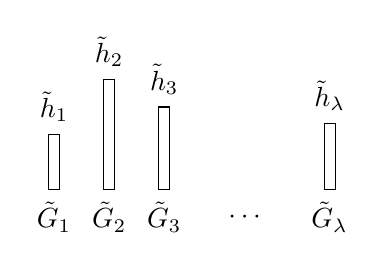
\begin{tikzpicture}[scale=0.7]
        \draw (0.0, 0) node {$\tilde{G}_1$}; \draw (0.0 - 0.1, 0.5) rectangle (0.0 + 0.1, 1.5); \draw (0.0, 1.5 + 0.5) node {$\tilde{h}_1$};
        \draw (1.0, 0) node {$\tilde{G}_2$}; \draw (1.0 - 0.1, 0.5) rectangle (1.0 + 0.1, 2.5); \draw (1.0, 2.5 + 0.5) node {$\tilde{h}_2$};
        \draw (2.0, 0) node {$\tilde{G}_3$}; \draw (2.0 - 0.1, 0.5) rectangle (2.0 + 0.1, 2.0); \draw (2.0, 2.0 + 0.5) node {$\tilde{h}_3$};
        \draw (3.5, 0) node {$\cdots $};
        \draw (5.0, 0) node {$\tilde{G}_\lambda $}; \draw (5.0 - 0.1, 0.5) rectangle (5.0 + 0.1, 1.7); \draw (5.0, 1.7 + 0.5) node {$\tilde{h}_\lambda $};
    \end{tikzpicture}
    \caption{Group partition}
    \end{center}
\end{figure}

} % End of ignore.


\section{Special Abilities and Battle Structure}
In this section we will discuss all battle or unit characteristics, modifiers, and abilities, that affect the normal course of the battle.

The key assumptions of the battle mechanics (as implemented by yours humbly) are as follows: damage can be fractional (or irrational even), hit points are always integer-valued. To allow for that, damage is always rounded \emph{up}. For example, when a group of units is hit with $31.416$ damage, the outcome would be exactly the same as if it was hit with $32$ damage.

Before the battle starts, there are two stages. First, each army's bonuses are applied. Next, each army's penalties are applied.
\begin{enumerate}
    \item Pre-battle bonus stage.
    \begin{enumerate}
        \item Explosive ammunition: every friendly unit in \emph{ranged} category gains \emph{attack weakest target} ability. Note that this will be ignored if the enemy army has \emph{intercept}.
        \item Accuracy bonus (additive): a given category of friendly unit's accuracy is increased by this amount. If the unmodified accuracy is $a$ and the accuracy bonus is $x$, the adjusted accuracy would be $(a + x)$, clipped to $[0.0, 1.0]$.
        \item Splash bonus (additive): a given category of friendly unit's splash chance is increased by this amount. If the unmodified splash chance is $s$ and the accuracy bonus is $x$, the adjusted splash chance would be $(s + x)$, clipped to $[0.0, 1.0]$.
        \item Minimum/maximum damage bonus (additive): a given category of friendly unit's minimum/maximum damage is increased by this amount. If the unmodified minimum/maximum damage is $d$ and the damage bonus is $x$, the adjusted damage would be $(d + x)$.
    \end{enumerate}
    \item Pre-battle penalty stage.
    \begin{enumerate}
        \item Boss health reduction (multiplicative): every enemy unit with \emph{boss} special ability will have a health penalty. If a boss unit has $h$ hit points and the boss health reduction is $x$, its actual hit points would become $\ceil{h \cdot (1 - x)}$.
        \item Dazzle: every enemy unit's accuracy is set to $0.0$.
        \item Intercept: every enemy unit is stripped of \emph{attack weakest target} ability.
    \end{enumerate}
\end{enumerate}

Some modifiers are applied during the battle. Suppose the current round is $n \geq 1$.
\begin{enumerate}
    \item Direct damage reduction (multiplicative): every enemy unit's damage is reduced by this amount. If a unit has $d$ damage and the direct damage reduction is $x$, the actual damage would become $\ceil{d \cdot (1 - x)}$.
    \item Tower damage reduction (multiplicative). If a friendly unit with \emph{tower bonus} special ability were to be hit with $d$ and the tower damage reduction is $x$, the actual inflicted damage would become $\ceil{d \cdot (1 - x)}$. Ignored if the attacking enemy unit has \emph{ignore tower bonus} ability.
    \item Frenzy bonus (multiplicative): every friendly unit's damage is multiplied by this amount. If the unmodified damage is $d$ and the frenzy bonus is $x$, the adjusted damage would be $\ceil{d \cdot (1 + x)^{(n - 1)}}$.
\end{enumerate}

\section{Timing}

Consider a battle between two armies\ignore{ $A_1$ and $A_2$}.
Let $T_f$, $T_d$, $T$, and $S$ be random variables
\begin{align*}
    T_f &= \{ \text{fighting time in rounds} \}, \quad
    T_d = \{ \text{destruction time in rounds} \}, \\
    T &= \{ \text{total time in rounds} \} = T_f + T_d, \\
    S &= \{ \text{loser's camp and surviving unit types} \}.
\end{align*}
%
Note that $\cond{T_d \ci T_f}{S}$, and write $T_d^s \triangleq (\cond{T_d}{S = s})$.

The result of fighting phase is the pair $(T_f, S)$. Given $s$, the observed value of $S$, the result of destruction phase is $T_d^s$.
Ultimately, we are interested in distributions of $T_f$, $T_d$, and $T$.


It is worth noting that destruction time, $T_s$, can be written as a stopping time. Let $m$ denote the number of surviving unit types, and write $s = \left( c, \{ u_i \} _{1 \le i \le m} \right)$. Let $h$ denote the number of hit points of the loser's camp, and $p_i$, $\overline{d_i}$, and $\underline{d_i}$ denote the accuracy, maximum, and minimum destruction damage of $u_i$. Let
\[
    D_t^s = \sum _{i = 1}^{m} \left( \overline{d_i} B_i^t + \underline{d_i} (1 - B_i^t) \right), \quad t \ge 1, \ignore{\quad D_0^s = 0,}
\]
be the damage per round inflicted by the survivors, where $\{ B_i^t \} _{1 \le i \le m, t \ge 1}$ are independent Bernoulli random variables, $B_i^t \sim \mathrm{Bernoulli}(p_i)$. Then
\[
    T_t^s = \inf \left\{ t \ge 0  \,:\, \sum _{k = 1}^t D_k^s \ge h \right\}.
\]

%+-----------------------------------------------------------------------------------------------+%
\section{Monte-Carlo simulations}

Let $n$ and $n_s$ denote the number of fighting phase simulations and destruction phase simulations, respectively. Then after simulating the fighting phase one can approximate
\begin{align}
    &\prob{P} (T_f = r, S = s) \approx \left( \sum _{i = 1} ^n \One \{ (t_{f, i}, s_i) = (r, s) \} \right) \Big\slash n, \quad
    \prob{P} (S = s) \approx \left( \sum _{i = 1} ^n \One \{ (t_{f, i}, s_i) = (\cdot , s) \} \right) \Big\slash n, \nonumber \\
    &\prob{P} (T_f = t) \approx \left( \sum _{i = 1} ^n \One \{ (t_{f, i}, s_i) = (t, \cdot ) \} \right) \Big\slash n. \label{eq:rounds_fight}
\end{align}
After simulating the destruction phase for every observed value of $s$, one gets
\begin{align}
    \prob{P} (T_d^s = t) &= \prob{P} (\cond{T_d = t}{S = s}) \approx \left( \sum _{i = 1} ^{n_s} \One \{ t_{d, i}^s = t \} \right) \Big\slash n_s, \nonumber \\
    \prob{P} (T_d = t) &= \sum _{s \in \mathcal{S}} \prob{P} (\cond{T_d = t}{S = s}) \, \prob{P} (S = s)
        = \sum _{s \in \mathcal{S}} \prob{P} (T_d^s = t) \, \prob{P} (S = s), \label{eq:rounds_destruct} \\
    \prob{P} (T = t) &= \sum _{r = 0}^t \prob{P} (T_f = r, T_d = t - r)
        = \sum _{s \in \mathcal{S}} \sum _{r = 0}^t \prob{P} (\cond{T_f = r, T_d = t - r}{S = s}) \, \prob{P} (S = s) \nonumber \\
        &= \sum _{s \in \mathcal{S}} \sum _{r = 0}^t \prob{P} (\cond{T_f = r}{S = s}) \, \prob{P} (\cond{T_d = t - r}{S = s}) \, \prob{P} (S = s) \nonumber \\
        &= \sum _{s \in \mathcal{S}} \sum _{r = 0}^t \prob{P} (T_f = r, S = s) \, \prob{P} (T_d^s = t - r) \label{eq:rounds_time}
\end{align}

% that's all folks
\end{document}

% $EOF$
%-------------------------------------------------------------------------------------------------%

